% le caratteristiche richieste dall'università sono elencate qui: https://stem.elearning.unipd.it/mod/book/view.php?id=234&chapterid=46#modalita
% 12pt: font richiesto dall'università
% twoside: i margini interni ed esterni sono scambiati per le pagine "a sinistra" e "a destra"
% openright: i capitoli cominciano in pagine dispari ("a destra")
% extreport: supporta 12pt
\documentclass[12pt,a4paper,twoside,openright]{extreport}

\usepackage{amsmath}                            % per avere più controllo sulle equazioni
\usepackage{csquotes}                           % per le citazioni
\usepackage{enumitem}                           % per avere più controllo sulle enumerazioni
\usepackage[
    a4paper,
    top=2cm,bottom=2cm,
    outer=2cm,inner=3cm,
    includeheadfoot
]{geometry}                                     % margini richiesti dall'università
\usepackage{graphicx}                           % per le immagini
\usepackage{icomma}                             % per separare le cifre decimali con una virgola
\usepackage{listings}                             % per il codice con la colorazione della sintassi
\usepackage[a-1a]{pdfx}                         % formato richiesto dall'università
\usepackage[output-decimal-marker={,}]{siunitx} % per le unità di misura
\usepackage{subcaption}                         % per le sottodidascalie
\usepackage{svg}                                % per inserire file SVG
\usepackage{mathtools}
\usepackage{algorithm}
\usepackage{algpseudocode}
\MakeRobust{\Call} % to use nested \Call

\usepackage[english]{babel}
\selectlanguage{english}

\usepackage[backend=bibtex,style=ieee]{biblatex}
\bibliography{bibliography}

\usepackage{setspace}
\onehalfspacing % interlinea richiesta dall'università

\sloppy % per evitare che il testo in \verb finisca oltre i margini

% questi valori vengono usati nella composizione del frontespizio
\title{Design and Evaluation of a Novel Heuristic for Delete-Free AI Planning}
\author{Andrea Stocco}
\date{GG/MM/AAAA}
\newcommand{\supervisor}{Prof. Domenico Salvagnin}

\usepackage{amsthm}
\theoremstyle{definition}
\newtheorem{definition}{Definition}[section]

\begin{document}
\pagenumbering{Roman}
\pagestyle{empty} % per le prime pagine, non mostrare il numero di pagina

\begin{titlepage}
	% solo il frontespizio deve essere simmetrico rispetto ai margini interno ed esterno
	\newgeometry{hmargin=2.5cm,vmargin=2cm}
	\begin{figure}
		\centering
		\begin{subfigure}[b]{0.4\textwidth}
			
\includegraphics[width=\textwidth]{images/logo_unipd}
		\end{subfigure}
		\hfill
		\begin{subfigure}[b]{0.3\textwidth}
			
\includegraphics[width=\textwidth]{images/logo_dei}
		\end{subfigure}
	\end{figure}

	\vspace*{\stretch{0.5}}

	\begin{center}
		\makeatletter % serve per poter usare \@...

		% NOTA: il Times New Roman non supporta il maiuscoletto.
		\textsc{Dipartimento di Ingegneria dell'Informazione}\\
		\vspace*{\stretch{0.1}}
		\textsc{Master Degree in Computer Engineering}

		\vspace*{\stretch{0.5}}
		\LARGE
		\textbf{\@title}

		\vspace*{\stretch{1}}
		\normalsize
		\begin{tabular*}{\textwidth}{l @{\extracolsep{\fill}} r}
			\textbf{Supervisor} & \textbf{Master Candidate} \\
			\supervisor       & \@author           \\
		\end{tabular*}

		\vspace*{\stretch{2}}
		\textsc{Academic Year 2024-2025} \\
		\vspace*{\stretch{0.1}}
		% Graduation Date\@date

		\makeatother % serve dopo \makeatletter
	\end{center}
	\restoregeometry
\end{titlepage}

\cleardoublepage

\vspace*{\stretch{1}}
\begin{flushright}
	\textit{To my family.}
\end{flushright}
\vspace{\stretch{4}}

\cleardoublepage

% NOTA: l'ambiente \abstract rimuove il numero della pagina e resetta il contatore delle pagine.
\begin{abstract}
	In this thesis, we present a new heuristic algorithm for solving delete-free AI planning problems.
Delete-free planning, where actions do not remove facts from the world state, offers a simplified yet
meaningful subset of classical planning. We propose an algorithm that estimates goal distances by
leveraging structural properties of delete-free domains. We compare its performance against
existing heuristic approaches on a range of benchmark problems. The evaluation demonstrates that our
method achieves competitive or improved results in terms of planning time and solution quality,
highlighting its potential for use in practical planning systems.

\end{abstract}
\cleardoublepage

\pagestyle{plain} % comincia a mostrare il numero di pagina

\tableofcontents
\cleardoublepage

\listoffigures
\cleardoublepage % per assicurarsi che la numerazione araba cominci col primo capitolo

\listoftables
\cleardoublepage

\listofalgorithms
\cleardoublepage

\pagenumbering{arabic}

\chapter{Introduction}
\label{ch:intro}
\textit{Automated Planning} (or AI Planning) is a core subfield of Artificial Intelligence.
A planning problem, in general terms, can be defined as the task of finding a sequence
of actions that leads from a given initial state to a desired goal state.
While multiple formal models exist for defining planning problems, this thesis
focuses on the \textit{$SAS^+$ formalism} defined in Definition \ref{def:sas+}

\begin{definition}[$\text{SAS}^+$ Planning Task]
	\label{def:sas+}
	A $\text{SAS}^+$ planning task is a 5-tuple $\Pi = \langle V, s_0, s_*, A \rangle$ with
	the following components:
	\begin{itemize}
		\item \(V\): finite set of state variables \(v\),
		      each with finite domain \textit{dom(v)}
		\item \(s_0\): variable assignment defining the initial state
		\item \(s_*\): partial variable assignment defining the goal
		\item \(A\): finite set of actions (or operators),
		      where each action $a \in A$ has the following components:
		      \begin{itemize}
			      \item Preconditions \textit{pre(a)}: partial variable assignment
			      \item Effects \textit{eff(a)}: partial variable assignment
			      \item Cost \textit{cost(a)}: non-negative real number
		      \end{itemize}
	\end{itemize}
\end{definition}

For an action $a \in A$ to be applicable, all of its preconditions
\textit{pre(a)} must be satisfied in the current state. Once applied, its effects
\textit{eff(a)} are used to update the current state accordingly.
In the simplified class of problems considered in this thesis—referred to as \textit{Delete-Free}—actions do not have any negative effects.
This means that once a fact becomes true in a state, it remains true in all subsequent states.
The solutions to planning problems are called \textit{plans}, and they are formally defined in Definition \ref{def:plan}

\begin{definition}[Plan]
	\label{def:plan}
	A plan for a planning problem is a sequence of actions occurring as labels on a path
	from the initial state to a goal state.
	The cost of a plan $\langle a_1, a_2, \dots, a_n \rangle$ is $\sum_{i = 1}^n cost(a_i)$.
	A plan is optimal if it has minimal cost.
\end{definition}

There exist optimal planners, such as \textit{Fast-Downward}, that are guaranteed to find the optimal solution to a given problem.
In contrast, this thesis focuses on \textit{heuristic} algorithms which—by design— do not
guarantee optimality, but aim to efficiently find near-optimal solutions in significantly less time.

TODO

\cleardoublepage

\chapter{Methodology}
\label{ch:methodology}
This chapter outlines the methodological approach used to compare the selected algorithms.
Several algorithms and variations were implemented in this thesis. Some
were chosen solely as baselines for the experiments, such as Random and Greedy.
As their names suggest, the former selects a random action at each iteration, while the latter
always chooses the action with the minimum cost.
The $h^{\max}$ heuristic \cite{bonet2001planning} is one of the most important
heuristics in Delete Free AI Planning problems. A revised version of this heuristic, incorporating
a pruning logic, is proposed in this work.
Additionally, a novel heuristic was developed, which assigns to each action the cost of the shortest path to reach the goal
state and then selects the action that is closest to the goal.\\
The experiments were conducted on a testbed containing 3,104 domain-independent instances.
Each algorithm was run on every instance with 10 different random seeds, resulting in 31,040 runs
per algorithm. A time limit of 60 seconds was set for each run.
All experiments presented in this thesis were conducted on a computing cluster maintained by the Operations Research group at the
Department of Information Engineering (DEI), University of Padova.
The cluster consists of 15 identical blades, each equipped with an Intel(R) Xeon(R) CPU E5-2623 v3 @ 3.00GHz, 16GB of RAM, and running Fedora 37.
The algorithms were compared in terms of solution cost, where a lower cost indicates a better solution.
To evaluate the effectiveness of the algorithms, a \textit{cumulative distribution plot} is used.
The concept of the primal gap, originally defined in the context of Mixed Integer Programming (MIP)
(see Definition \ref{def:primalgap}) \cite{berthold2013measuring}, is adapted here to quantify the quality of solutions across algorithms.

\begin{definition}[Primal Gap]
	\label{def:primalgap}
	Let \~x be a solution for a problem, and $\text{\~x}_{opt}$ be an optimal (or best known)
	solution for that problem. We define the primal gap $\gamma \in \left[0, 1\right]$ of \~x as follows:
	\begin{equation*}
		\gamma\left(\text{\~x}\right)\coloneqq\begin{cases}
			0,                                                                                                                            & \text{if $\lvert c^T\tilde{x}_{opt}\rvert$ = $\lvert c^T\tilde{x}\rvert$ = 0}, \\
			1,                                                                                                                            & \text{if $c^T\tilde{x}_{opt} \cdot c^T\tilde{x} < 0$},                         \\
			\frac{\lvert c^T\tilde{x}_{opt} - c^T\tilde{x} \rvert}{max \{\lvert c^T\tilde{x}_{opt} \rvert, \lvert c^T\tilde{x} \rvert\}}, & \text{else}.
		\end{cases}
	\end{equation*}
\end{definition}

An algorithm that finds the best solution for a given instance will exhibit a primal gap of zero.
For all other algorithms, the primal gap approaches zero as the solution quality approaches the best known,
and approaches one as it deviates further from it.
For each algorithm, a cumulative distribution plot is generated by plotting the percentage of instances
on which the algorithm has a primal gap below a given threshold. A more detailed explanation of this analysis will be provided in the following sections.

\cleardoublepage

\chapter{Proposed Approaches}
\label{ch:heuristics}
Heuristics are algorithms to determine a near-optimal solution to a problem. In certain scenarios,
exact methods aren't able to provide the optimal solution in a reasonable amount of time or they can't find it
at all. In contrast, a heuristic is generally capable of offering a solution that is more or less close to
the optimal one.
While there is no assurance regarding the optimality of the provided solution, it may still be considered
acceptable in some instances.
This chapter focuses on explaining the algorithms developed, while the following one presents their evaluation.\\
Before diving into the topic, it is important to understand some of the functions used by all the algorithms.
An action, in order to be eligible for application, must have all its preconditions satisfied in the current state.
If even one precondition is not satisfied, the entire action cannot be applied.
Additionally, applying an action means adding its effects to the current state.
The pseudocode for this function is shown in Algorithm \ref{alg:apply}.

\begin{algorithm}
	\caption{Apply}
	\label{alg:apply}
	\hspace*{0.5em} \textbf{Output}: $newState$
	\begin{algorithmic}[1]
		\Procedure{apply}{$currentState, actionToApply$}
		\State $newState \gets \Call{copy}{currentState}$
		\ForAll{$fact \in actionToApply.effects$}
		\If{$fact \notin newState$}
		\State $newState \gets newState \cup \{fact\}$
		\EndIf
		\EndFor
		\State \textbf{return} $newState$
		\EndProcedure
	\end{algorithmic}
\end{algorithm}

\section{Random}
This is the simplest algorithm implemented, and it is used as a baseline for the evaluation.
At each iteration, it applies a random action from the applicable ones.
It is not a sophisticated or informed solution but this strategy can be useful
in some cases because, by chance, a good plan may be found.
Algorithm \ref{alg:random} shows the pseudocode for it.

\begin{algorithm}
	\caption{Random}
	\label{alg:random}
	\hspace*{0.5em} \textbf{Output}: $solution$
	\begin{algorithmic}[1]
		\Procedure{random}{$planningTask$}
		\State $currentState \gets planningTask.initialState$
		\State $solution \gets [\ ]$ \Comment{Initialize empty solution}
		\While {$planningTask.goalState \not\subseteq currentState$}
		\State $possibleActions \gets \{a \in A \mid pre(a) \subseteq currentState\}$
		\If {$\Call{empty}{possibleActions}$}
		\State \textbf{return} $failure$ \Comment{Infeasible problem}
		\EndIf
		\State $actionToApply \gets \Call{randomChoice}{possibleActions}$
		\State $currentState \gets \Call{apply}{currentState, actionToApply}$
		\State \Call{append}{$solution$, $actionToApply$}
		\EndWhile
		\State \textbf{return} $solution$
		\EndProcedure
	\end{algorithmic}
\end{algorithm}

It is important to notice that if \textit{posissibleActions} is empty, then
a solution to the planning task cannot exist. As said in Chapter \ref{ch:intro},
the problems are Delete-Free|once a fact becomes true in the current state, it remains
true until the end.
Therefore, if there are no actions to apply, it does not mean that the algorithm has reached
a dead end that could be avoided by applying different actions in a different order.
Rather, it indicates that no sequence of actions can lead to the goal state, and therefore no plan exists.
The natural evolution of this approach is to avoid choosing randomly the next action to apply and, instead, use
a strategy to select the action that is more likely to lead to a better plan.

\section{Greedy}
A greedy algorithm is a heuristic that attempts to find an optimal solution by selecting the locally
best possible choice at each iteration. For instance, in our case, the next action to apply will
always be the one with the minimum cost. In the case of a tie, a random action among those with the same cost
will be chosen.
Algorithm \ref{alg:greedy} shows the pseudocode for this algorithm. The omitted parts are identical to those in Algorithm \ref{alg:random}.

\begin{algorithm}
	\caption{Greedy}
	\label{alg:greedy}
	\hspace*{0.5em} \textbf{Output}: $solution$
	\begin{algorithmic}[1]
		\Procedure{greedy}{$planningTask$}
		\State \dots
		\State $possibleActions \gets \{a \in A \mid pre(a) \subseteq currentState\}$
		\If {$\Call{empty}{possibleActions}$}
		\State \textbf{return} $failure$
		\EndIf
		\State $actionToApply \gets \Call{minimumCostAction}{possibleActions}$
		\State \dots
		\EndProcedure
	\end{algorithmic}
\end{algorithm}

Instead of randomly choosing the next action to apply, here the action with minimum cost is always selected.
For this and all subsequent algorithms, if multiple eligible actions share the same minimum (heuristic) cost,
one of them is selected at random.

\section{Revised Max Heuristic}
\label{sec:hmax}
The max heuristic is one of the most well-known delete-relaxation heuristics in the literature.
It is an \textit{admissible} heuristic, meaning that it never overestimates the cost of reaching the goal.
It assigns an heuristic cost to each action based on Equation \ref{eq:hmax} and \ref{eq:cost}

\begin{equation}
	\label{eq:hmax}
	h_{max}\left(p;s\right) \coloneqq \begin{cases}
		0                                                                & \text{if $p \in s$} \\
		\text{min}_{a \in O\left(p\right)}\left[h\left(a;s\right)\right] & \text{otherwise}
	\end{cases}
\end{equation}

where $h_{max}\left(p;s\right)$ stands for an estimate of the cost of achieving the fact \textit{p} from
the current state \textit{s}, $O\left(p\right)$ is the set of actions $\{a \in A \mid p \in \textit{eff(a)}\}$, and

\begin{equation}
	\label{eq:cost}
	h\left(a;s\right) \coloneqq cost(a) + \text{max}_{q \in pre\left(a\right)} \left[h(q, s)\right]
\end{equation}

stands for the cost of achieving the preconditions of an action \textit{a} and applying it.\\
The idea behind the use of this heuristic is similar to that of the greedy approach.
While in the greedy approach the action with the minimum actual cost is chosen, in this case,
the action with the minimum heuristic cost is selected at each iteration.
This thesis presents an implementation of the max heuristic that goes a step further.
By definition, any action applicable in the current state has a heuristic cost equal to
its own cost, since all its preconditions are satisfied|regardless of whether the action is
actually useful for reaching the goal state or not.
The implemented version performs a technique called \textit{pruning}, which consists of assigning
an infinite cost to useless actions|indicating that these actions are not helpful in finding a good plan.
As a result, such actions are effectively excluded from consideration when selecting the next action to apply,
while the remaining ones retain their correct heuristic cost.
The pseudocode for this algorithm is presented in Algorithm \ref{alg:hmax} and \ref{alg:greedyhmax}.

\begin{algorithm}
	\caption{Max Heuristic}
	\label{alg:hmax}
	\hspace*{0.5em} \textbf{Output}: $minHcost$
	\begin{algorithmic}[1]
		\Procedure{hmax}{$currentState, fact$}
		\If {$fact \in currentState$}
		\State \textbf{return} 0 \Comment{Base case}
		\EndIf
		\State $actions \gets \{a \in A \mid fact \in \textit{eff(a)}\}$ \Comment{Get all the actions having \textit{fact} as effect}
		\If {$\Call{empty}{actions}$}
		\State \textbf{return} $+\infty$ \Comment{The fact is unreachable}
		\EndIf
		\State $minHcost \gets +\infty$
		\ForAll{$action\in actions$}
		\State $maxCost \gets 0$
		\ForAll {$pre \in action.preconditions$}
		\State $maxCost \gets \Call{max}{maxCost, \Call{hmax}{currentState, pre}}$
		\EndFor
		\State $action.hCost \gets action.cost + maxCost$
		\State $minHcost \gets \Call{min}{minHcost, action.hCost}$
		\EndFor
		\State \textbf{return} $minHcost$
		\EndProcedure
	\end{algorithmic}
\end{algorithm}

\begin{algorithm}
	\caption{Greedy Search with Max Heuristic}
	\label{alg:greedyhmax}
	\hspace*{0.5em} \textbf{Output}: $solution$
	\begin{algorithmic}[1]
		\Procedure{greedyHmax}{$planningTask$}
		\State \dots
		\ForAll {$a \in A$}
		\State $a.hCost \gets +\infty$ \Comment{Initialize actions' heuristic cost}
		\EndFor
		\State $estimatedCost \gets 0$
		\ForAll {$goal \in planningTask.goalState$}
		\State $estimatedCost \gets \Call{max}{estimatedCost, \Call{hmax}{currentState, goal}}$
		\EndFor
		\State $possibleActions \gets \{a \in A \mid pre(a) \subseteq currentState\}$
		\If {$\Call{empty}{possibleActions}$}
		\State \textbf{return} $failure$
		\EndIf
		\State $actionToApply \gets \Call{minimumHcostAction}{possibleActions}$
		\State \dots
		\EndProcedure
	\end{algorithmic}
\end{algorithm}

Starting from each fact in the goal state, \verb|HMAX| is invoked to perform backward cost propagation.
Through this process, actions that do not contribute to achieving the goal will implicitly retain their initial cost of $+\infty$,
effectively marking them as useless. When selecting the next action to apply, any action with infinite cost is ignored,
and the one with the lowest heuristic cost among the remaining options is chosen.\\
Figure \ref{fig:hmax_scheme} illustrates the behaviour of the max heuristic without the pruning technique.
Each circle represents a state in the planning task, with $s_i$ as initial state (in blue) and $s_g$ as goal state (in green).
Edges denote actions, each labeled with its heuristic cost. Although the edges in the figure are undirected, each action conceptually connects
a state that must be satisfied as a precondition to a resulting state that becomes true as an effect. For example, action $a_2$ is applicable in
$s_i$, and its effect is to reach $s_2$.  For simplicity, all actions have a uniform actual cost of 1.
When the heuristic is applied from the initial state, the actions $a_1$, $a_2$, and $a_3$ are all deemed applicable and assigned heuristic costs
equal to their actual cost. However, since multiple actions have the same cost, the tie-breaking mechanism (e.g., random choice) may lead the planner
to select a suboptimal branch|such as choosing $a_1$ or $a_3$| which does not contribute toward reaching the goal efficiently.

\begin{figure}[ht]
	\centering
	\def\svgwidth{0.75\linewidth}
	\input{images/hmax.pdf_tex}
	\caption{Behaviour of the max heuristic without pruning}
	\label{fig:hmax_scheme}
\end{figure}

Figure \ref{fig:hmax_pruning_scheme} shows the same planning instance, but this time using the max heuristic augmented with the pruning technique.
Here, actions that do not contribute to achieving the goal are implicitly assigned a heuristic cost of $+\infty$. As a result, the planner deterministically
selects $a_2$ from the initial state, as it is the only action with a finite cost.
The heuristic is recomputed after each action, updating costs based on the new state. This guided progression ensures that only goal-relevant actions are
considered. For this instance, the pruning-enhanced heuristic always leads to the optimal plan: $a_2$, $a_6$, $a_{11}$, $a_{14}$.

\begin{figure}[ht]
	\centering
	\def\svgwidth{0.75\linewidth}
	\input{images/hmax_pruning.pdf_tex}
	\caption{Behaviour of the max heuristic with pruning}
	\label{fig:hmax_pruning_scheme}
\end{figure}

As previously mentioned, any action that can be applied from
the current state will always have a heuristic cost equal to its actual cost.
Therefore, this algorithm can be seen as a greedy + pruning approach: it selects the next action based on the action's cost,
while discarding useless actions.
To observe the true behavior of the proposed algorithm, it should ideally be used within the context of the \verb|A*| algorithm,
a well-known search strategy that combines actual cost from the start with a heuristic estimate to the goal.
Specifically, \verb|A*| selects actions by minimizing the function $f(n) = g(n) + h(n)$, where $g(n)$ is the cost
required to reach node $n$, and $h(n)$ is the estimated cost to reach the goal state from $n$.
\verb|A*| selects actions based on the sum of these two values, leading to optimal solutions when an admissible heuristic, such as \verb|HMAX|, is used.
However, since \verb|A*| was not implemented in this thesis, an alternative approach was used to evaluate the algorithm's actual performance.

\section{Max Heuristic + Lookahead}
As mentioned in the previous section, the presented algorithm can be considered a greedy + pruning approach,
since the full potential of the heuristic cannot be exploited|the heuristic cost of the applicable actions is always equal
to the actions' actual cost.
To evaluate its performance, a new version of the heuristic is proposed.
Instead of selecting the action with the minimum cost, the algorithm tries each possible action,
recomputes the \verb|HMAX| value for each resulting state, and finally applies the action that leads to the state with the lowest
new heuristic value.
The pseudocode for this approach is shown in Algorithm \ref{alg:lookahead} and \ref{alg:hmaxlookahead}.

\begin{algorithm}
	\caption{Lookahead}
	\label{alg:lookahead}
	\hspace*{0.5em} \textbf{Output}: $actionToApply$
	\begin{algorithmic}[1]
		\Procedure{lookahead}{$currentState, possibleActions$}
		\ForAll{$action\in possibleActions$}
		\State $newState \gets \Call{apply}{currentState, action}$
		\State $estimatedCost \gets 0$
		\ForAll {$goal \in planningTask.goalState$}
		\State $estimatedCost \gets \Call{max}{estimatedCost, \Call{hmax}{newState, goal}}$
		\EndFor
		\State $action.hCost \gets action.hCost + estimatedCost$
		\EndFor
		\State $actionToApply \gets \Call{minimumHcostAction}{possibleActions}$
		\State \textbf{return} $actionToApply$
		\EndProcedure
	\end{algorithmic}
\end{algorithm}

\begin{algorithm}
	\caption{Max Heuristic with Lookahead}
	\label{alg:hmaxlookahead}
	\hspace*{0.5em} \textbf{Output}: $solution$
	\begin{algorithmic}[1]
		\Procedure{hmaxLookahead}{$planningTask$}
		\State \dots
		\State $estimatedCost \gets 0$
		\ForAll {$goal \in planningTask.goalState$}
		\State $estimatedCost \gets \Call{max}{estimatedCost, \Call{hmax}{currentState, goal}}$
		\EndFor
		\State $possibleActions \gets \{a \in A \mid pre(a) \subseteq currentState\}$
		\If {$\Call{empty}{possibleActions}$}
		\State \textbf{return} $failure$
		\EndIf
		\State $actionToApply \gets \Call{lookahead}{currentState, possibleActions}$
		\State \dots
		\EndProcedure
	\end{algorithmic}
\end{algorithm}

The algorithm "looks ahead" at the heuristic cost of the state resulting from each possible action,
and then applies only the action that appears to be the most convenient.

\section{Novel Heuristic}
\label{sec:shortestpath}
In this section, a completely new approach is introduced. As discussed in Section \ref{sec:hmax},
the modified version of the max heuristic ultimately behaves like a greedy + pruning algorithm, limiting its effectiveness.
Here, we aim to use the same backward propagation mechanism, but with a different heuristic cost assigned to each action.
The core idea is to assign each action a cost that estimates its actual distance to the goal.
Specifically, the cost assigned to an action corresponds to the cost of the \textit{shortest path} to reach a fact in the goal state.
The mathematical formalism is presented in Equations \ref{eq:sp} and \ref{eq:spcost}:

\begin{equation}
	\label{eq:sp}
	h_{sp}\left(p;s_*\right) \coloneqq \begin{cases}
		0                                                                    & \text{if $p \in s_*$} \\
		\text{min}_{a \in O\left(p\right)}\left[h_a\left(a;s_*\right)\right] & \text{otherwise}
	\end{cases}
\end{equation}

Here, $h_{sp}\left(p;s_*\right)$ denotes the estimated cost of achieving a fact in the goal state $s_*$, starting from
fact \textit{p}. The set $O\left(p\right)$ represents the actions that produce \textit{p} as an effect,
that is, $O\left(p\right) = \{a \in A \mid p \in \textit{eff(a)}\}$. The function $h_a\left(a;s_*\right)$ is
defined as follows:

\begin{equation}
	\label{eq:spcost}
	h_a\left(a;s_*\right) \coloneqq cost(a) + \text{min}_{q \in \textit{eff}\left(a\right)} \left[h_{sp}\left(q;s_*\right)\right]
\end{equation}

This espression estimates the cost of achieving a fact in the goal state $s_*$ by applying
action \textit{a}. The heuristic cost of an action is defined as its own cost plus the minimum estimated cost among its effects.
In this way, each action is assigned a heuristic cost corresponding to the cost of the shortest path to reach
a fact in the goal state.
The actual implementation of this algorithm uses a \textit{priority queue} to ensure an
efficient and iterative computation. The pseudocode is presented in Algorithm \ref{alg:sp}.

\begin{algorithm}
	\caption{Shortest Path Heuristic}
	\label{alg:sp}
	\hspace*{0.5em} \textbf{Output}:
	\begin{algorithmic}[1]
		\Procedure{shortestPath}{$currentState, goalState$}
		\State $factCosts \gets \{+\infty, \dots, +\infty\}$ \Comment{Initialize facts' cost to $+\infty$}
		\State $pq\gets \{\}$ \Comment{Empty priority queue}
		\ForAll {$goal \in goalState$}
		\State $factCosts[goal] \gets 0$
		\State $\Call{push}{pq, goal, 0}$
		\EndFor
		\While {$!\Call{empty}{pq}$}
		\State $fact \gets \Call{pop}{pq}$ \Comment{Get the fact having minimum cost}
		\If {$fact \in currentState$}
		\State \textbf{continue} \Comment{Do not propagate the cost}
		\EndIf
		\State $actions \gets \{a \in A \mid fact \in \textit{eff}\left(a\right)\}$
		\ForAll {$action \in actions$}
		\State $newCost \gets action.cost + factCosts[fact]$
		\If {$newCost >= action.hCost$}
		\State \textbf{continue}
		\EndIf
		\State $action.hCost = newCost$
		\ForAll {$pre \in action.preconditions$}
		\If {$newCost < factCosts[pre]$}
		\State $factCosts[pre] \gets newCost$
		\If {$\Call{has}{pq, pre}$}
		\State $\Call{change}{pq, pre, newCost}$
		\Else
		\State $\Call{push}{pq, pre, newCost}$
		\EndIf
		\EndIf
		\EndFor
		\EndFor
		\EndWhile
		\EndProcedure
	\end{algorithmic}
\end{algorithm}

The priority queue internally maintains the facts ordered by increasing cost.
Each time a fact is removed from the queue, it is the one with the minimum heuristic cost.
The heuristic cost of each action having the removed fact as an effect is then updated accordingly,
and all of its preconditions are subsequently inserted into the queue.
In this way, all useful actions will be assigned a cost equal to the shortest path to reach a fact in
the goal state, while useless actions will retain an infinite cost.
The usage of this algorithm is analogous to what was presented in Algorithm \ref{alg:greedyhmax}.

\cleardoublepage

\chapter{Results}
\label{ch:results}
This chapter presents an evaluation of the algorithms introduced in Chapter \ref{ch:heuristics}.
To assess their performance, a cumulative distribution plot was used.
This type of plot shows the percentage of instances for which an algorithm found a plan with a
primal gap below the threshold indicated on the x-axis.
The best algorithm is the one whose curve lies above all the others.
The plots presented in the following sections will help illustrate this concept.
As described in Chapter \ref{ch:methodology}, each algorithm was run on every instance in the
testbed 10 times, each with a different random seed.
There are 3,104 instances, so each algorithm was executed a total of 31,040 times.
To limit execution time, each run was given a time limit of 60 seconds. The instances
come from different domains; some are very large in terms of number of actions, while others are
relatively small.
Additionally, since some algorithms are more efficient than others, not all the instances
were solved by every algorithm. Table \ref{tab:timelimit} shows, for each algorithm,
the number of instances it was able to solve within the time limit.

\begin{table}[h!]
	\centering
	\begin{tabular}{|l|r|}
		\hline
		\textbf{Heuristic}        & \textbf{Not found per timelimit} \\
		\hline
		Random                    & 1123                             \\
		Greedy                    & 1076                             \\
		Greedy + Pruning          & 1714                             \\
		Max Heuristic + Lookahead & 9199                             \\
		Shortest Path             & 851                              \\
		\hline
	\end{tabular}
	\caption{Number of instances not solved within the time limit (out of 31,040 total instances).}
	\label{tab:timelimit}
\end{table}

By simply examining this table, we can identify the most effective algorithms.
The lookahead process is computationally expensive, resulting in approximately one-third of the instances not being solved.
In contrast, the efficient implementation of the shortest path heuristic appears to be the most capable,
solving the highest number of instances.

\section{Random vs Greedy vs Greedy + Pruning vs Shortest Path}
This section presents an evaluation of four planning strategies, ranging from uninformed to increasingly informed approaches:
random, greedy, greedy + pruning, and shortest path.
Random and greedy exhibit similar efficiency, as both are able to solve a large number of instances. Greedy + pruning is
slightly slower but employs a strategy with the potential to yield higher-quality solutions. Ultimately, the shortest path approach
solves the highest number of instances. The next step is to evaluate the quality of the solutions produced by each strategy.
Figure \ref{fig:rgps} presents the cumulative distribution plot for the evaluated algorithms.

\begin{figure}[h!]
	\centering
	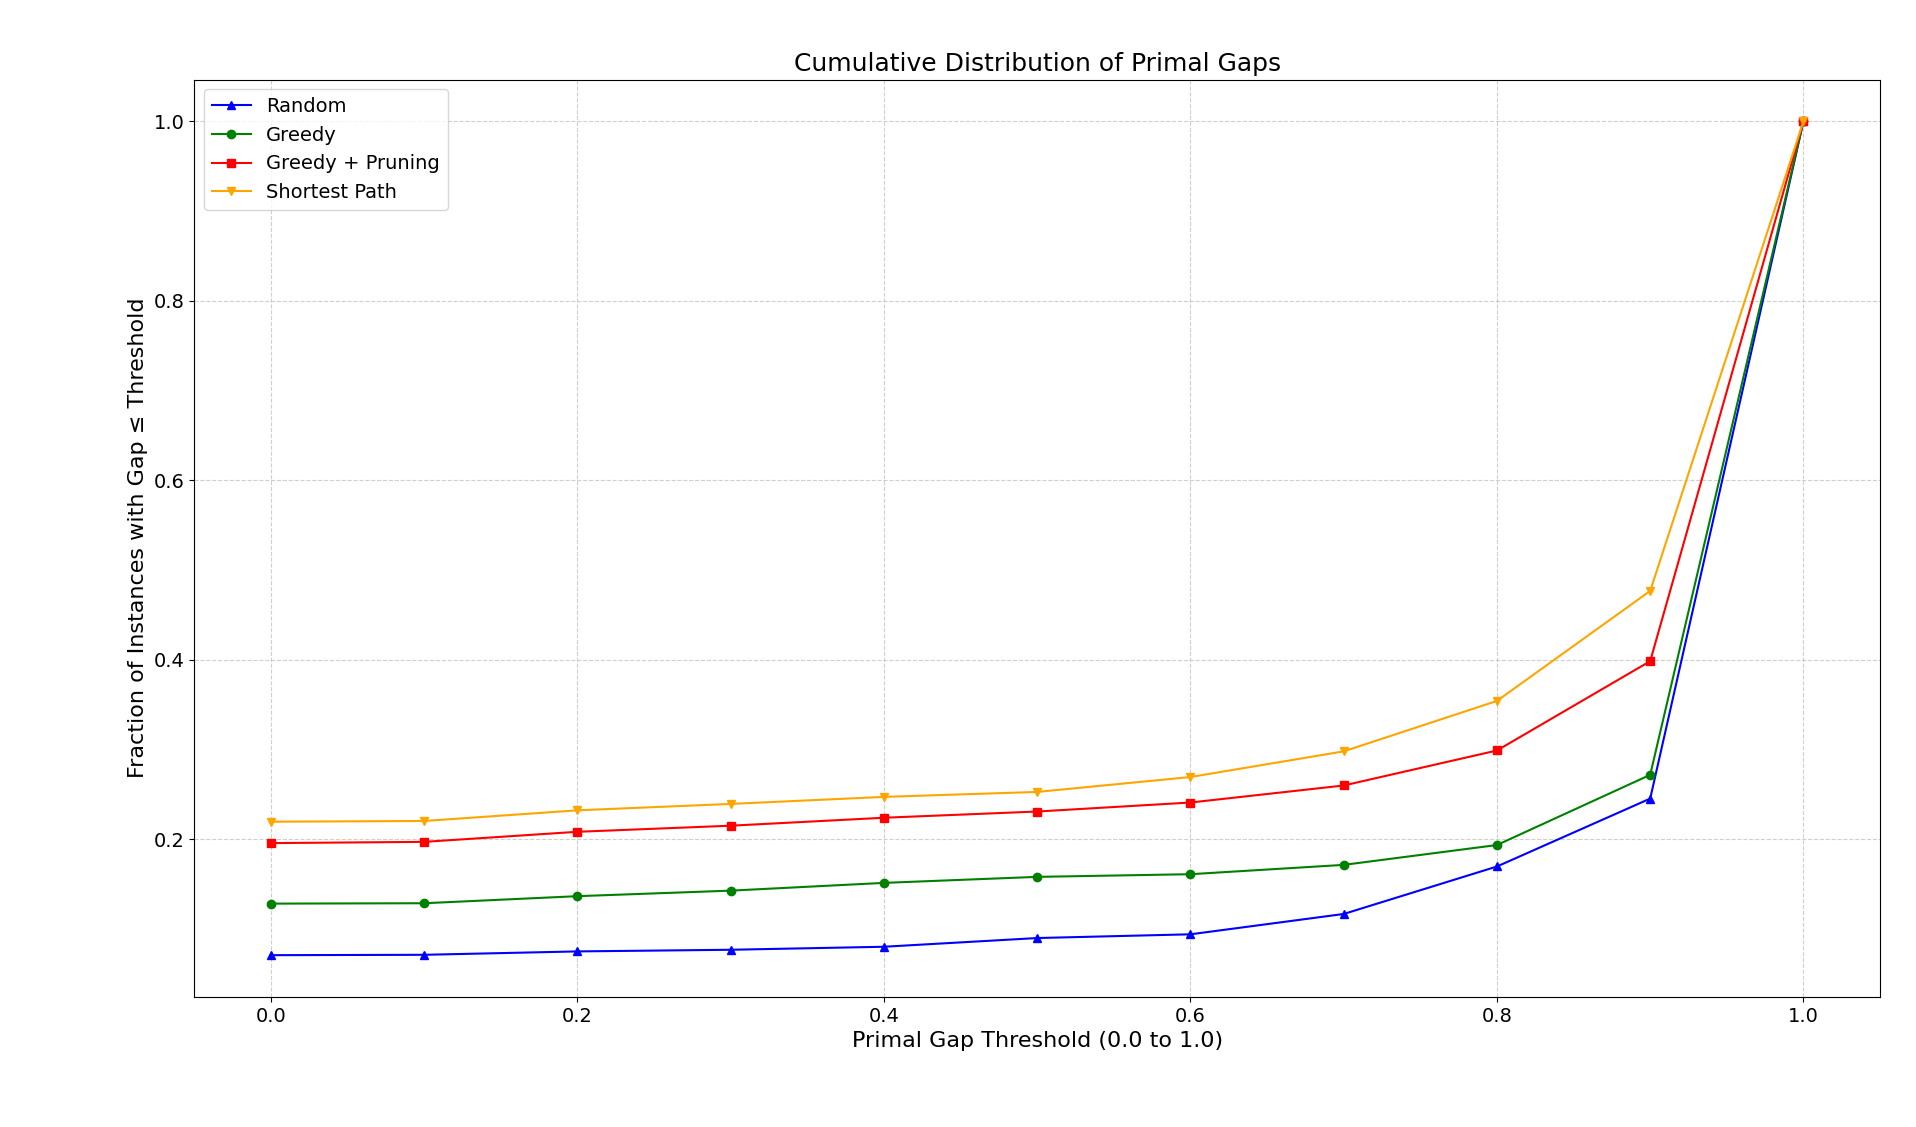
\includegraphics[width=\textwidth]{images/algs0124.png}
	\caption{Cumulative distribution plot for Random, Greedy, Greedy + Pruning, and Shortest Path strategies.}
	\label{fig:rgps}
\end{figure}

For instance, to better interpret the plot, consider the greedy strategy: the point on its curve corresponding to
a primal gap threshold of 60\% is close to 20\%. This indicates that it achieves a solution with a primal gap less than
or equal to 60\% in approximately 20\% of the problem instances.
Conversely, the shortest path strategy found the best known solution (i.e., a primal gap of 0\%) in approximately
25\% of the instances.
Now that the plot has been properly explained, it is possible to identify the most effective heuristic.
The curve that remains above all the others represents the best-performing strategy, as it indicates that the corresponding
algorithm consistently found solutions within the primal gap thresholds for a larger number of instances.
As expected, random and greedy stategies typically do not produce high-quality plans. Pruning the useless actions appears to be
an effective strategy, as it allows the planner to discard actions that are known to be unhelpful whenever multiple
options with the same cost are available.
Shortest Path builds on pruning by also estimating the distance to the goal for each action, resulting in a more
informed and effective selection of actions to include in the plan.

\section{Greedy + Pruning vs Hmax + Lookahead}
As shown in the previous section, pruning proves to be an effective strategy.
The initial idea was to combine pruning with the max heuristic. However, due to the nature of the heuristic’s definition,
this approach effectively reduces to a greedy + pruning strategy. To better evaluate its potential,
a lookahead mechanism was implemented to assess whether combining pruning with the max heuristic could lead
to a more promising solution. This section presents an evaluation of the performance of these two algorithms.
The lookahead process is computationally expensive; as a result, the algorithm fails to find a plan for approximately
one-third of the instances. Figure \ref{fig:algs23} presents the cumulative distribution plot comparing the performance
of these two algorithms.

\begin{figure}[h!]
	\centering
	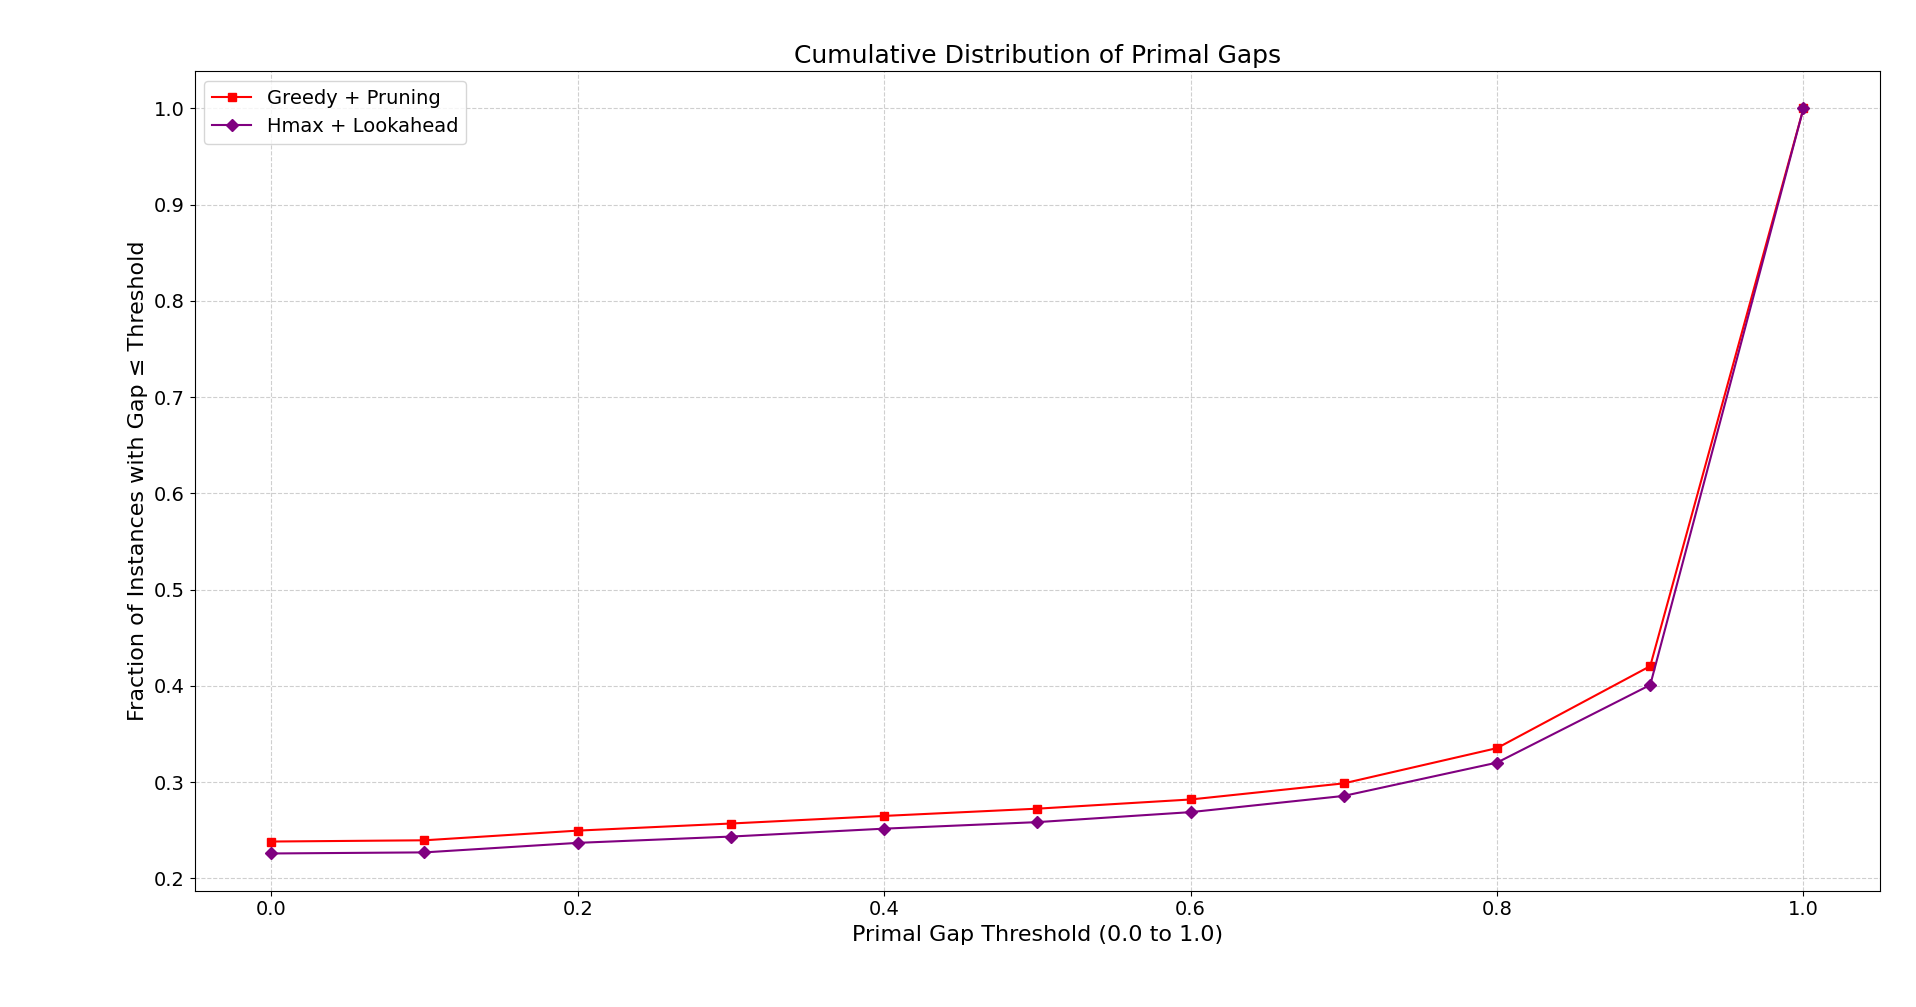
\includegraphics[width=\textwidth]{images/algs23.png}
	\caption{Cumulative distribution plot for Greedy + Pruning, and Max Heuristic + Lookahead strategies.}
	\label{fig:algs23}
\end{figure}

Unfortunately, this plot alone cannot definitively answer which of the two algorithms produces better-quality plans.
The high number of unsolved instances by the hmax + lookahead algorithm can skew the results: greedy + pruning may
appear superior simply because it solves more instances, not necessarily because it generates better plans.
There is no guarantee that the plans found by greedy + pruning are of higher quality than those returned by hmax + lookahead.
Figure \ref{fig:algs234_solved_all} shows a comparison between the algorithms, considering only the instances that were successfully
solved by all of them.

\begin{figure}[h!]
	\centering
	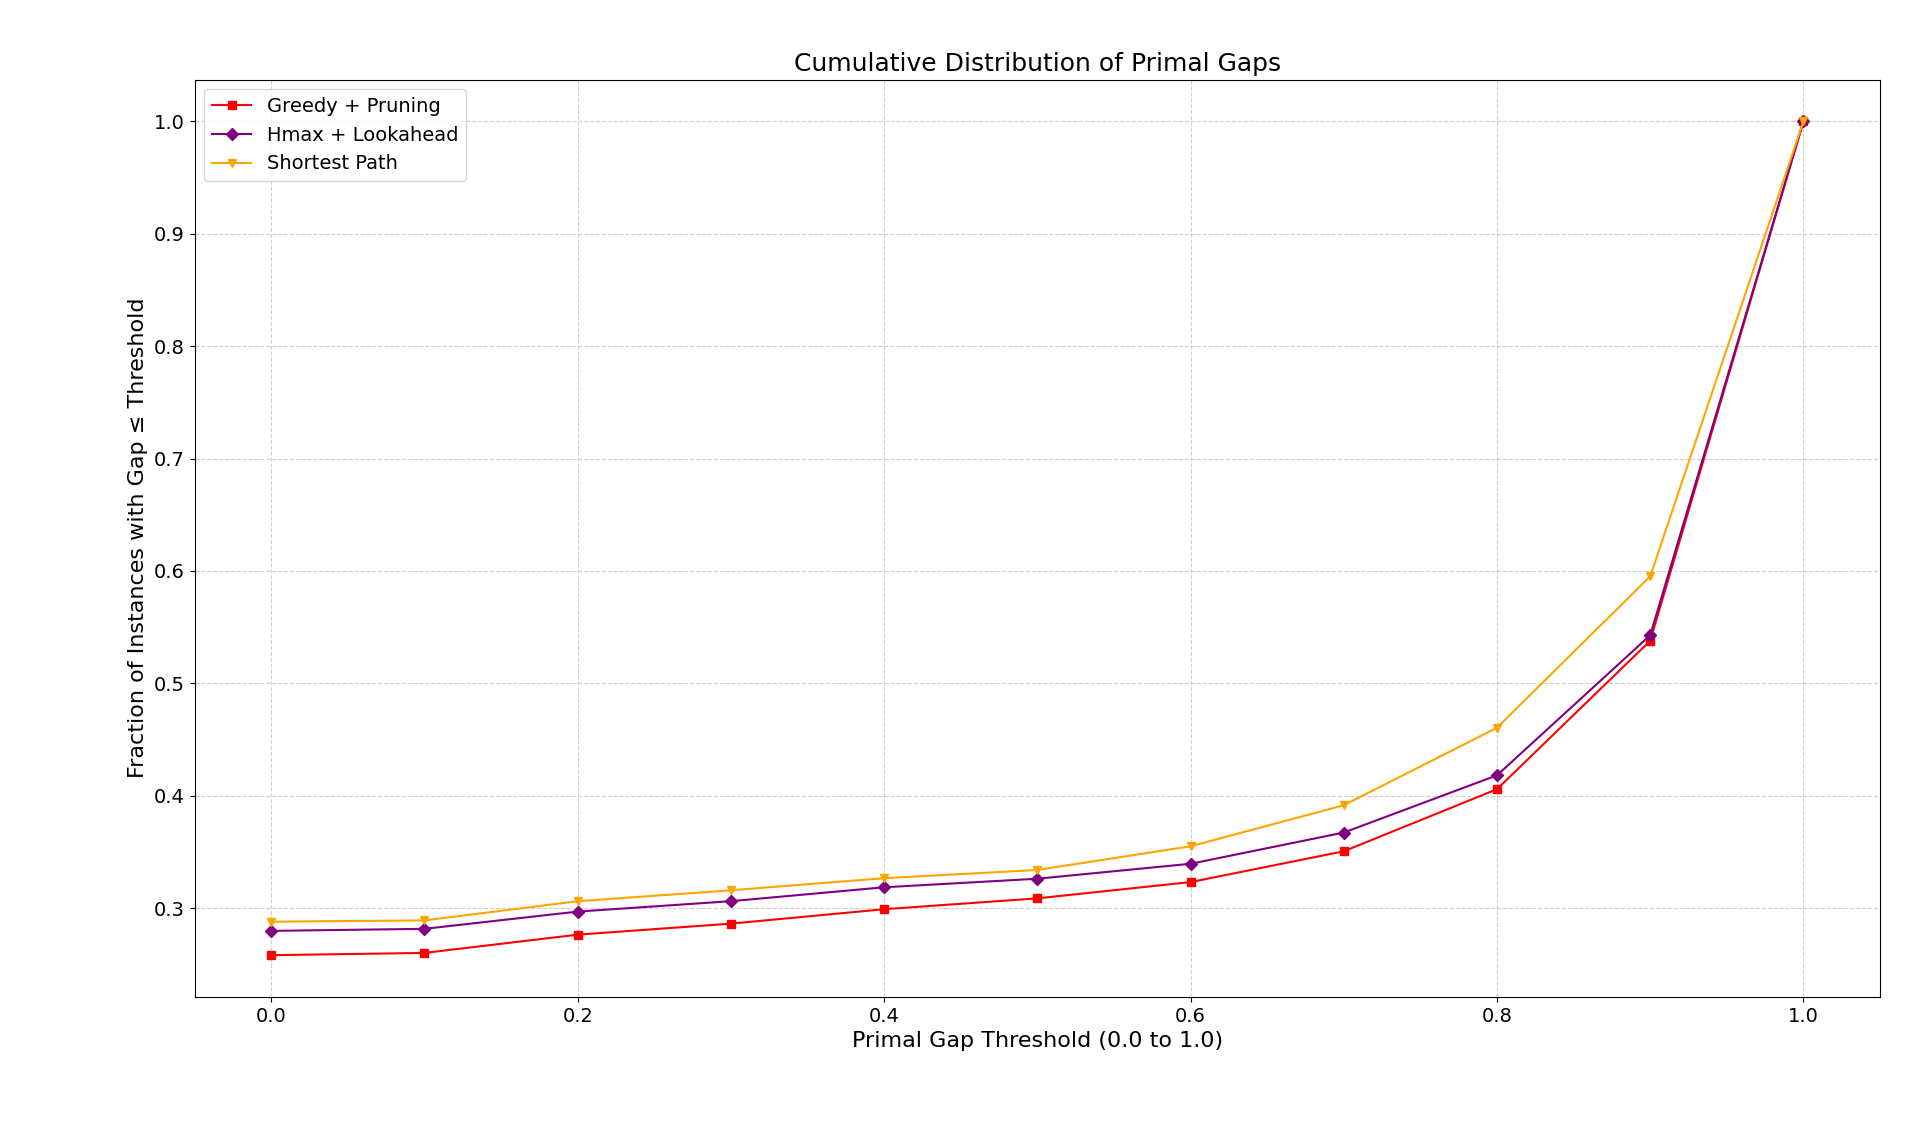
\includegraphics[width=\textwidth]{images/algs234_solved_all.png}
	\caption{Cumulative distribution plot for Greedy + Pruning, Max Heuristic + Lookaheado, and Shortest Path strategies,
		considering only the instances solved by all of them.}
	\label{fig:algs234_solved_all}
\end{figure}

The curve for shortest path is included as a reference. Focusing only on the instances solved by all the presented algorithms
is particularly valuable: in this case, the curves are not skewed by instances that some strategies failed to solve.
This allows us to assess only the quality of the generated plans. From this comparison, it is evident that shortest path
is the best-performing algorithm overall—both in terms of solution quality and the number of problems it can solve.
Additionally, the performance of hmax + lookahead, which surpasses that of greedy + pruning, confirms that pruning combined
with max heuristic can be an effective strategy when paired with a lookahead mechanism.
Although Lookahead remains a slow algorithm, these results suggest that the revised version of the max heuristic|enhanced
with a pruning mechanism|has the potential to produce high-quality solutions if used within a more powerful search strategy
like \verb|A*|.

\section{Different Versions of Backward Propagation}
As explained in Section \ref{sec:shortestpath}, the core idea behind the algorithm is to back-propagate the estimated cost
of reaching the goal state from its constituent facts to those in the current state. Previously, an algorithm was introduced
that propagates the minimum cost among an action's effects—effectively computing the shortest path to the goal.
With minimal modification, alternative strategies can be explored, such as propagating the \textit{maximum effect cost} or the
\textit{sum of all effect costs} to preceding actions. These variations are evaluated in Figure \ref{fig:backprop} to determine which
propagation strategy yields better results.

\begin{figure}[h!]
	\centering
	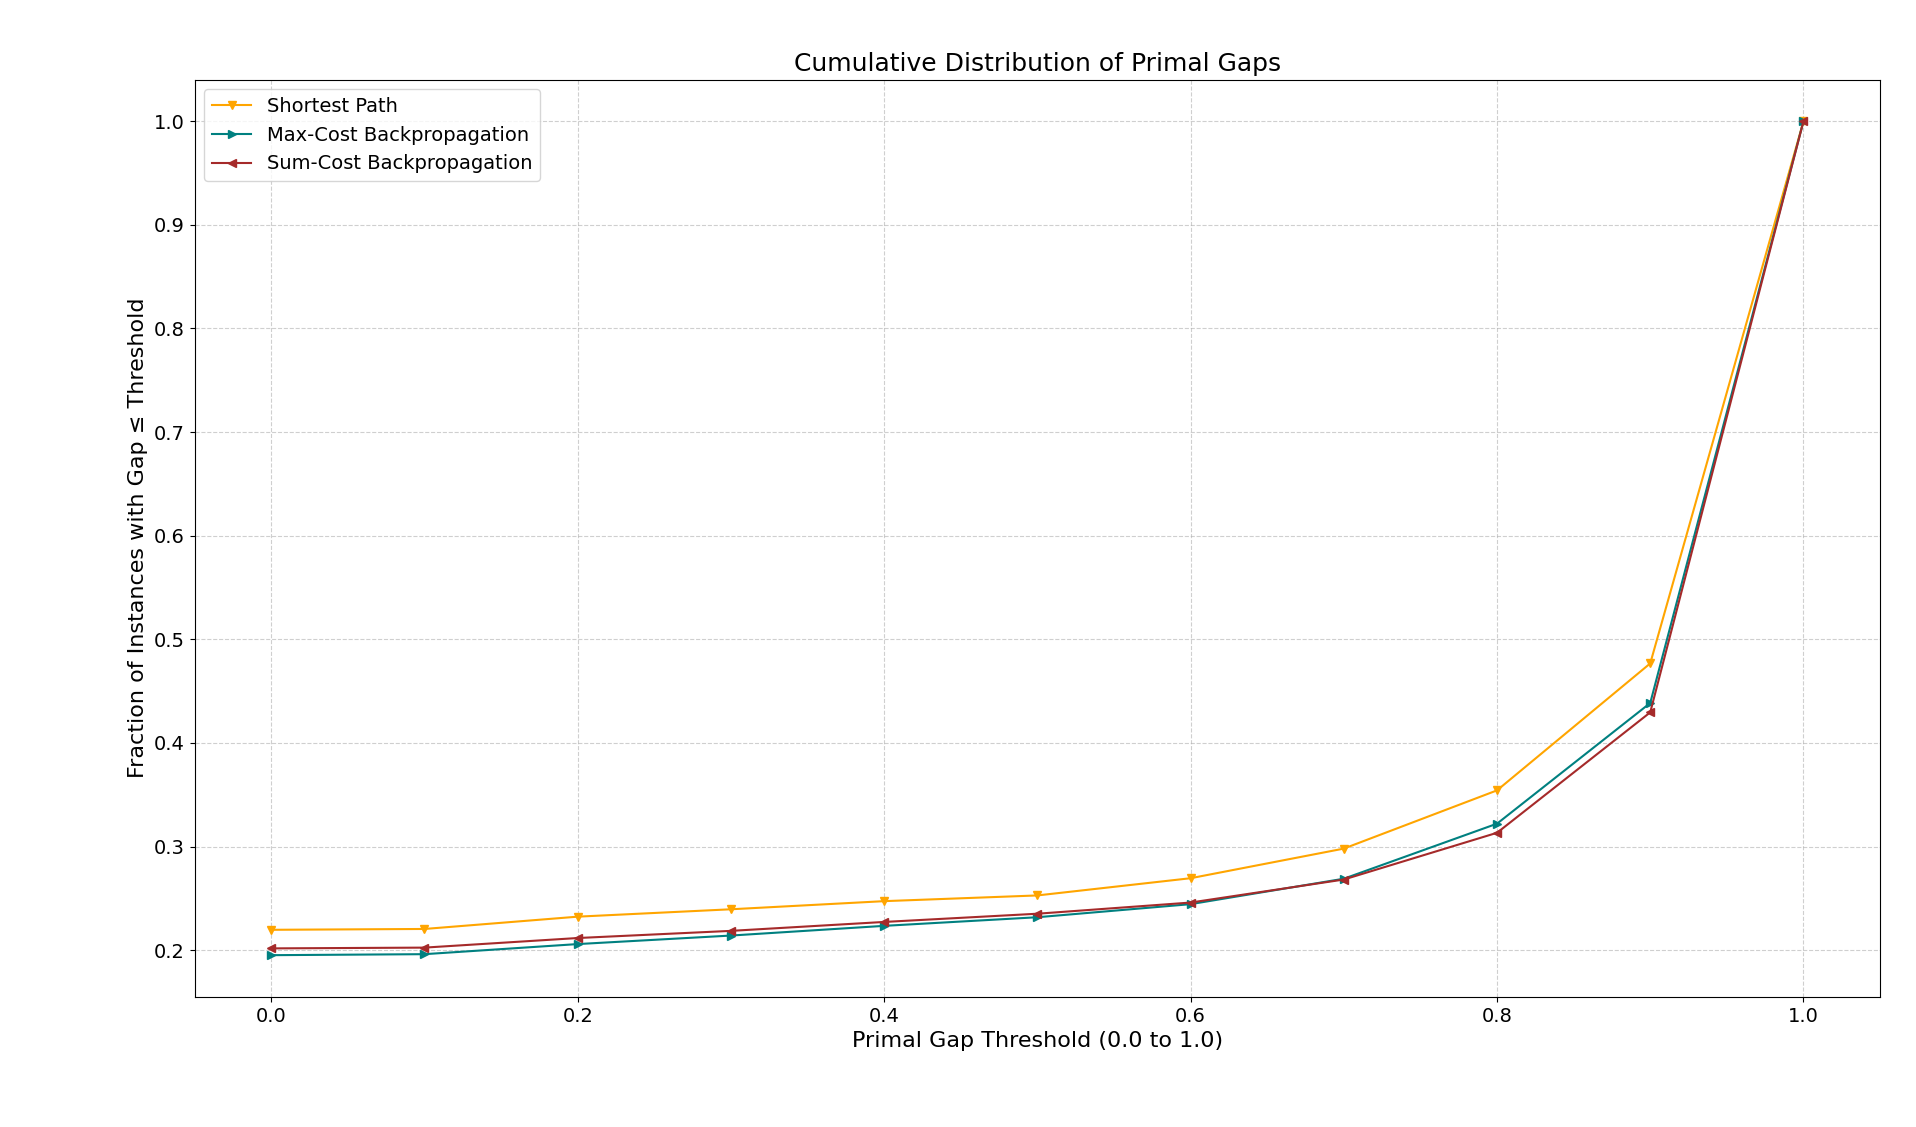
\includegraphics[width=\textwidth]{images/algs456.png}
	\caption{Cumulative distribution plot for different backpropagation strategies}
	\label{fig:backprop}
\end{figure}

Back-propagating the maximum cost among an action’s effects can be interpreted as assigning the action a cost based on
the worst-case path to the goal state. Conversely, back-propagating the sum of the effects' costs reflects a perspective
where all possible outcomes of the action contribute to estimating the distance to the goal. Each approach offers a different
trade-off between pessimism and comprehensiveness in cost estimation.
The Shortest Path heuristic continues to deliver the best performance overall. In contrast, both the max-cost and sum-cost
backpropagation strategies exhibit similar behavior, with only marginal differences between them.

\cleardoublepage

\chapter{Conclusions}

\cleardoublepage

\nocite{planning-tutorial}
\printbibliography[heading=bibintoc]
\end{document}
